
\section{Hydrogen Test Bench}%
\label{sec:h2 design}%
\emph{The hydrogen test bench design is based on the On-Off controlled battery architecture selected in Chapter~\ref{chap:concept design}. This section presents the detailed design of the hydrogen test bench and the selection of its individual subsystems and components. First, an overview of the complete system architecture is provided, followed by the design considerations and trade-off analyses that led to the final component selections.}

\subsection*{System Overview}
% The hydrogen test bench consists of the following main subsystems:

% \begin{itemize}
%     \item Hydrogen supply and regulation subsystem
%     \item Fuel cell subsystem
%     \item Power management and control subsystem
%     \item Load emulation subsystem
% \end{itemize}
The hydrogen test bench is an integrated system capable of emulating the operation of the hydrogen based power generation and feed system as completely as possible. The test bench is designed to experimentally evaluate the interaction between hydrogen generation, pressure regulation, electrical power management and propulsion loading under dynamic operating conditions. Figure~\ref{fig:h2_overview} shows a high-level overview of this system.

\begin{figure}[htp]
    \centering
    \begin{tikzpicture}[node distance=4cm]

        % Nodes
        \node (supply) [process] {Hydrogen Supply \\ \& Regulation};

        \node (fc) [component, right of=supply] {Fuel Cell};

        \node (pm) [process, right of=fc] {Power Management \\ \& Control};

        \node (battery) [component, below of=pm, yshift=1.5cm] {Battery};

        \node (load) [component, right of=pm] {Load Emulation};

        % Hydrogen flow
        \draw[arrow] (supply) -- (fc);

        % Electrical power flow
        \draw[arrow] (fc) -- (pm);
        \draw[arrow] (pm) -- (load);
        \draw[arrow, <->] (pm) -- (battery);

        % Control feedback
        \draw[arrow, dashed] (supply.south) |- ($(pm.south)+(0,-0.8)$) -- (pm.south);

    \end{tikzpicture}

    \caption{High-level overview of the hydrogen test bench architecture}
    \label{fig:h2_overview}
\end{figure}

Figure~\ref{fc:h2 test} shows the fluidic architecture of the hydrogen supply system. Hydrogen is supplied from a pressurized storage tank and routed through the CGG equivalent, which emulates the behaviour and internal volume of the cool gas generator. The hydrogen then passes through the pressure regulation system before entering the fuel cell.

Figure~\ref{fc:electric test} shows the electrical architecture of the test bench. Electrical power generated by the fuel cell is regulated using a buck converter and supplied to a shared 24~V power bus connected to the battery and propulsion load. The battery acts as an energy buffer during transient load conditions, while the relay-based On-Off controller regulates the fuel cell power draw based on the pressure measured in the hydrogen buffer volume. Power meters and sensors throughout the system provide the measurements required to analyse system performance and validate the proposed architecture.

\clearpage
\begin{figure}[htp]
    \centering

    \begin{tikzpicture}[node distance=2cm]
        % \draw[help lines] (0, 6) grid (15,-6);

        \node (tank) [volume] at (6,0) {\ce{H2} Tank};
        \draw (3,0) pic[rotate=180] {pressure regulator};
        \pic (qr) at (0,0) {quickrelease};
        \node (valve) [manual valve] at (-0.5, 3) {};
        \draw[thick] (qr-in) .. controls +(-1,0) and +(-1,0) .. (valve.west);

        \coordinate (cggloc) at (2,3);
        \aircgg{cggloc}
        \pic (filter) at (cggloc) {filter};
        \pic (regulator2) at (10,3) {pressure regulator};
        \node[draw, thick, minimum width=2cm, minimum height=2cm] (fc) at (13,3) {Fuel Cell};

        \draw[thick] (tank) -- (qr-out);
        \draw[thick] (valve) -- (filter-in);
        \draw[thick] (cggloc) ++(5,0) -- (fc);
    \end{tikzpicture}

    \caption{Fluidics of the Hydrogen Test Setup}
    \label{fc:h2 test}
\end{figure}

\begin{figure}[htp]
    \centering
    \begin{tikzpicture}[node distance=3cm, power/.style=red, data/.style=blue, core/.style={fill=blue!25}]
        % \draw[help lines] (0, 0) grid (15,-6);

        \node (sensor) [component, anchor=west] {Pressure Sensor};
        \node (rpi) [component, below of=sensor, yshift=-1cm, core] {Raspberry Pi};
        \node (buck2) [component, below of=rpi, yshift=1cm] {Buck Converter};

        \node (pm1) [component, right of=sensor, xshift=3cm] {Power Meter};
        \node (fc) [component, above of=pm1, yshift=-1cm, core] {Fuel Cell};
        \node (buck1) [component, right of=pm1] {Buck Converter};
        \node (relay) [component, right of=buck1] {Relay};

        \node (pm2) [component, below of=pm1, yshift=-1cm] {Power Meter};
        \node (battery) [component, left of=pm2, core] {Battery};

        \node (pm3) [component, below of=buck1, yshift=-1cm] {Power Meter};
        \node (drone) [component, right of=pm3, core] {Motor};

        \draw (sensor.west) ++ (0,-2) node (i2c) [component, minimum width=14cm, text width=4cm, anchor=west] {Data Bus (\iic)};
        \draw (battery.west) ++ (0,-2) node (24v) [component, minimum width=11cm, text width=4cm, anchor=west] {Power Bus (24 V)};

        \draw[arrow, power] (fc) -- (pm1);
        \draw[arrow, power] (pm1) -- (buck1);
        \draw[arrow, power] (buck1) -- (relay);
        \draw[arrow, power] (relay.east) -- ++(1,0) |- (24v);
        \draw[arrow, data, <-] (relay.south) -- ++(0,-1);
        \draw[arrow, data, ->] (pm1.south) -- ++(0,-1);

        \draw[arrow, power, <->] (pm2) -- (battery);
        \draw[arrow, power, <->] (pm2.south) -- ++(0,-1);
        \draw[arrow, data, ->] (pm2.north) -- ++(0,1);

        \draw[arrow, power] (pm3) -- (drone);
        \draw[arrow, power, <-] (pm3.south) -- ++(0,-1);
        \draw[arrow, data, ->] (pm3.north) -- ++(0,1);

        \draw[arrow, data] (sensor.south) -- +(0, -1);
        \draw[arrow, power] (24v) -- (buck2);
        \draw[arrow, power] (buck2) -- (rpi);
        \draw[arrow, data] (battery.north) -- +(0, 1);
        \draw[arrow, data, <->] (rpi.north) -- +(0, 1);

        \draw (relay.north) ++(-0.7,1) coordinate (legend);

        \draw (legend) -- ++(0.5, 0) [arrow, data];
        \draw (legend) ++(1.2,0) node[align=left, text width=1cm] {Data};
        \draw (legend) ++(0,0.5) -- ++(0.5,0) [arrow, power];
        \draw (legend) ++(1.2,0.5) node[align=left, text width=1cm] {Power};
    \end{tikzpicture}


    \caption{Electronics of the Hydrogen Test Setup}
    \label{fc:electric test}
\end{figure}
% \todo{Picture of real world system}


\begin{figure}[htp]
    \centering
    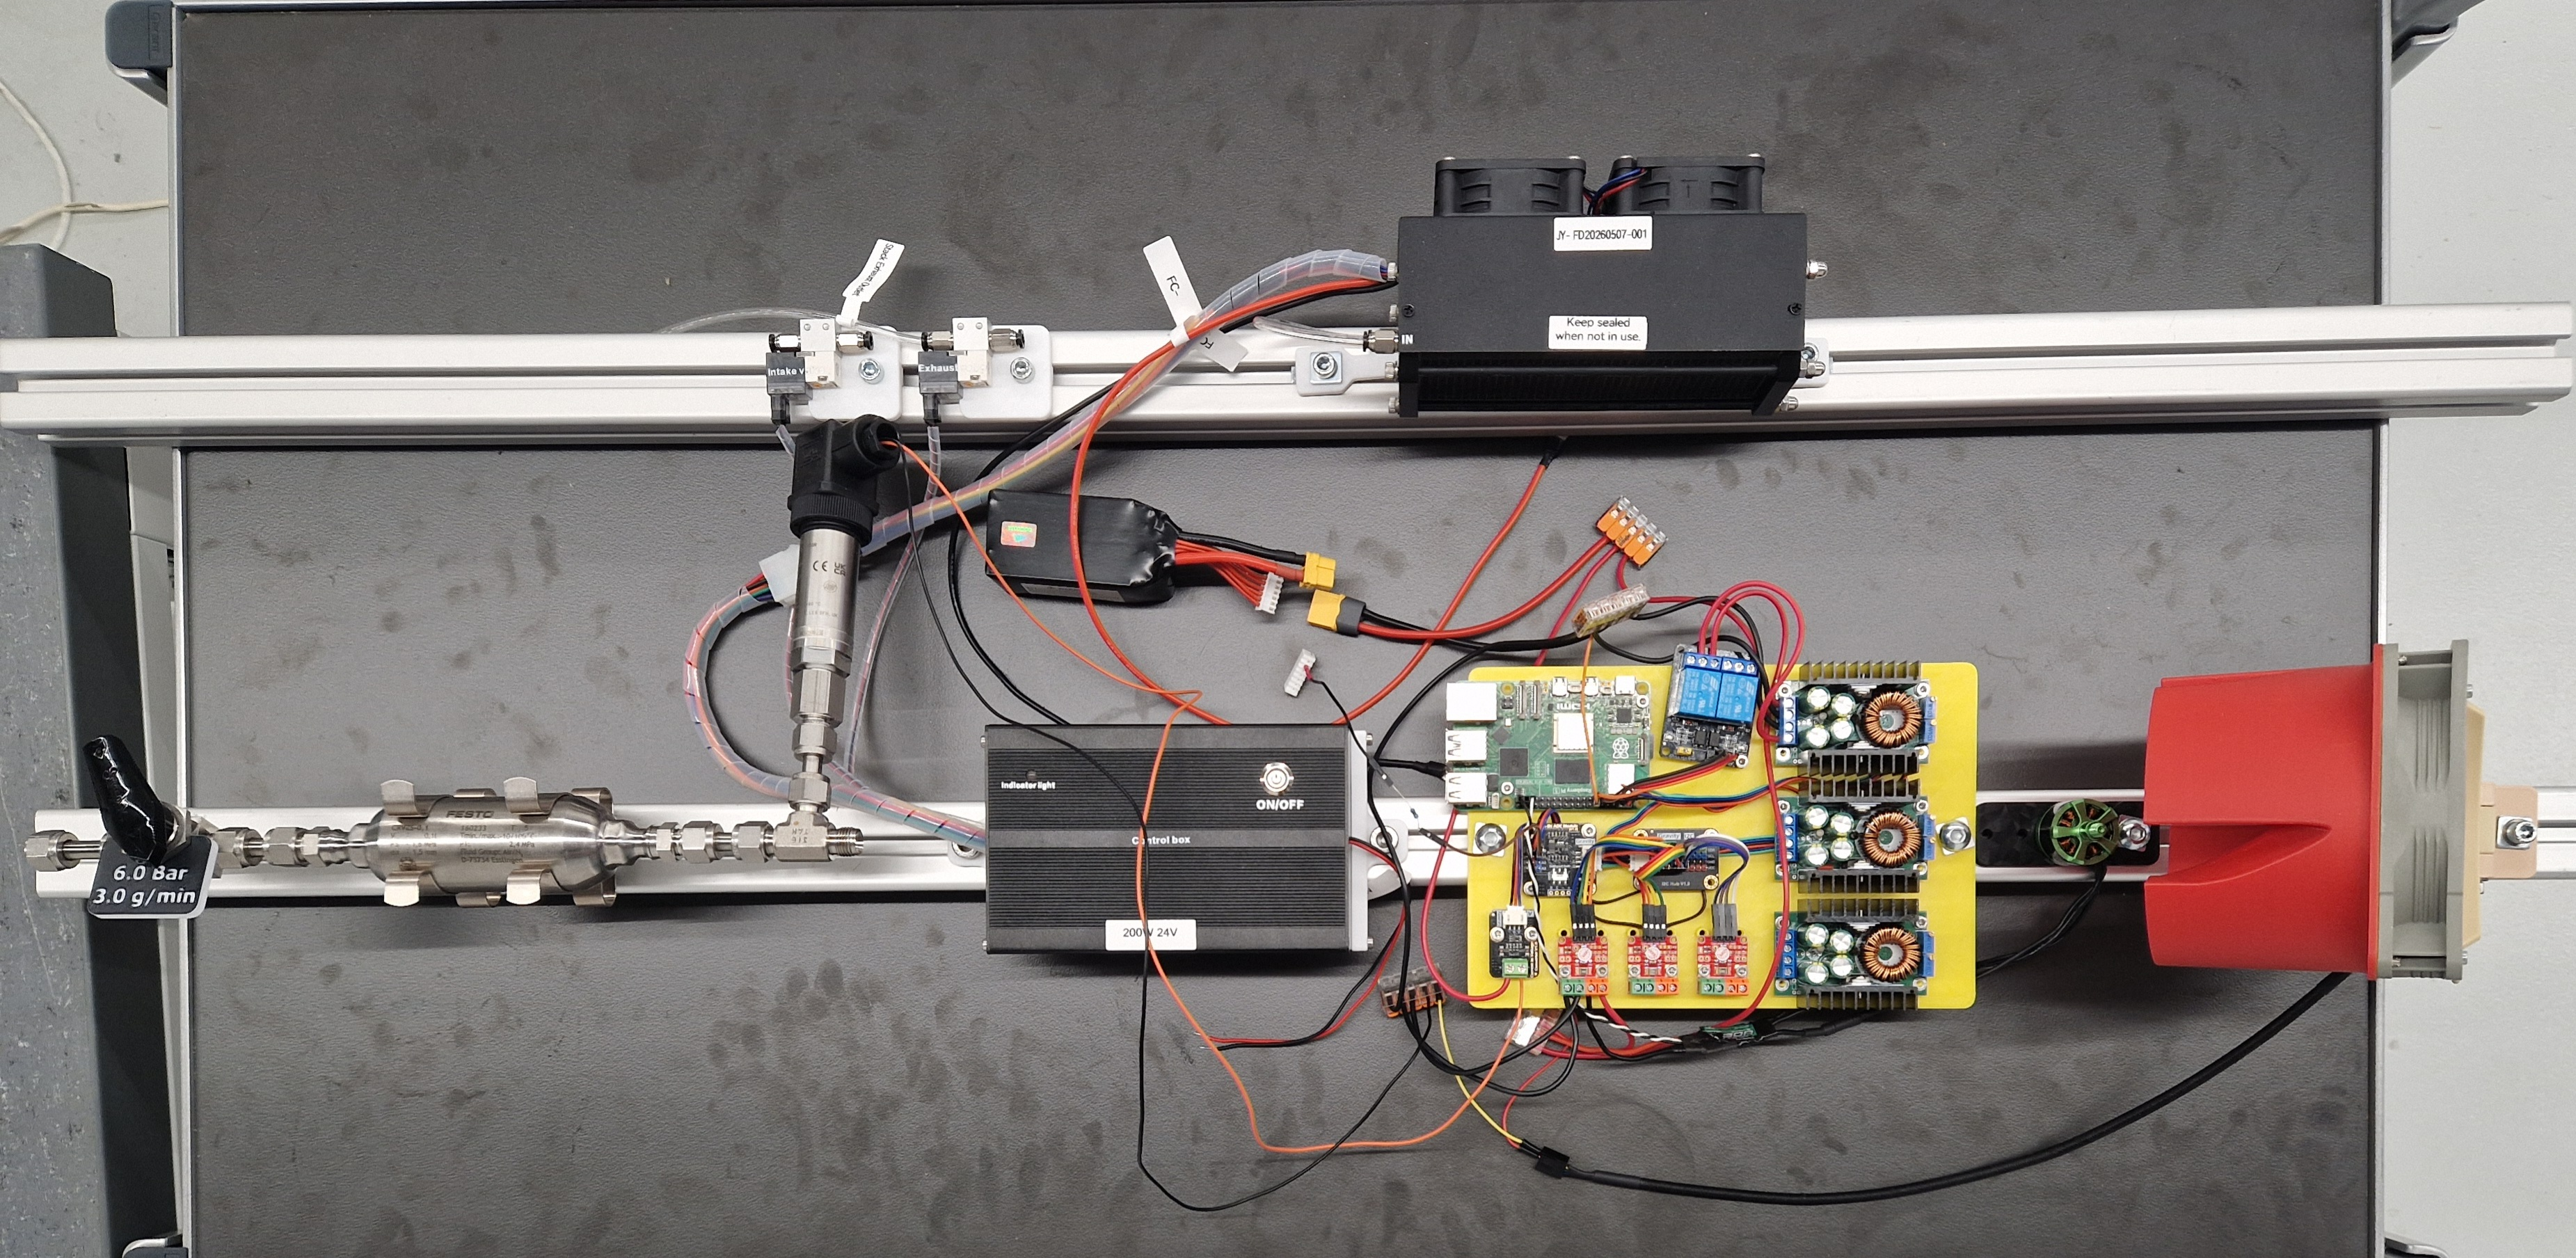
\includegraphics[width=\textwidth]{media/rl h2 setup.jpg}
    \caption{Picture of the Hydrogen Test Setup}
    \label{fig:rl h2 test}
\end{figure}

\clearpage



\subsection*{Fuel Cell Selection}

The fuel cell is the primary power generation component of the hydrogen test bench and therefore strongly influences the overall system behaviour. The selected fuel cell must be capable of delivering sufficient electrical power to emulate the expected UAV operating conditions while remaining compatible with the available hydrogen supply and electrical power management system.

Several commercially available PEM fuel cells were considered for integration into the test bench. The selection was primarily based on the following criteria:

\begin{itemize}
    \item Output power capability
    \item Availability and delivery time
    \item Cost
    \item Compatibility with the intended operating voltage range
    \item Ease of integration into the test setup
\end{itemize}

Table~\ref{tab:fc tradeoff} compares the considered fuel cell systems.

\begin{table}[htp]
    \begin{tabularx}{\textwidth}{lXXX}
        \toprule
        \textbf{Name}                                     & \textbf{IE-SOAR 800} & \textbf{H-200} & \textbf{H2Gatech} \\
        \midrule
        \textbf{Image}                                    &
        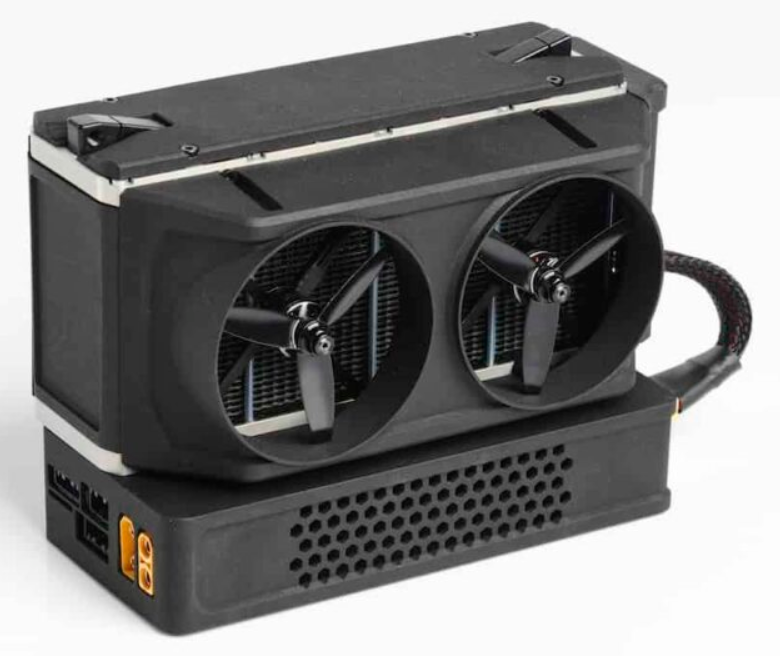
\includegraphics[width=\linewidth]{media/fc1.png} &
        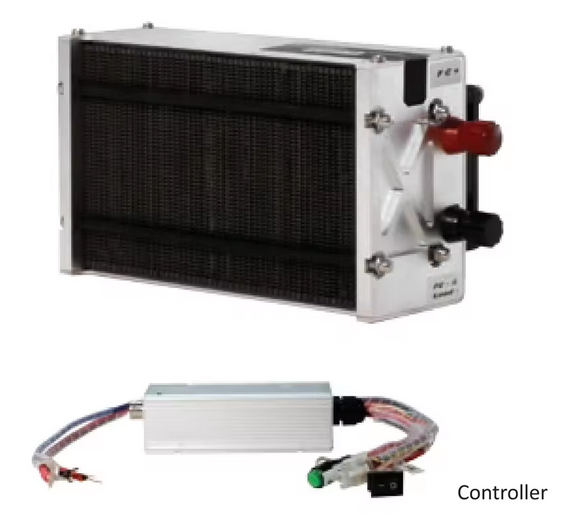
\includegraphics[width=\linewidth]{media/fc2.png} &
        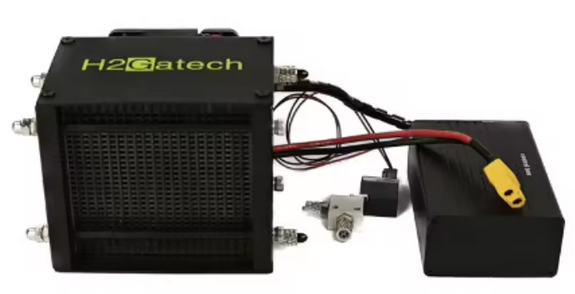
\includegraphics[width=\linewidth]{media/fc3.png}                                                             \\
        \midrule
        \textbf{Power}                                    & 800 W                & 200 W          & 200 W             \\
        \textbf{Price}                                    & Quote                & € 1164         & € 715             \\
        \textbf{Shipping}                                 & Unknown              & $\pm$1 month   & 5--20 Days        \\
        \bottomrule
    \end{tabularx}
    \caption{Tradeoff table of different fuel cells}
    \label{tab:fc tradeoff}
\end{table}
Although the IE-SOAR 800 offers significantly higher power output, insufficient information regarding pricing and delivery time made it unsuitable for this project. The H-200 and H2Gatech systems both satisfy the minimum power requirements of the test bench. Due to its significantly lower cost and shorter delivery time, the H2Gatech fuel cell was selected for integration into the hydrogen test bench.
\clearpage


\subsection*{Hydrogen Supply and Regulation}
In the hydrogen based power generation and feed system, the hydrogen supply shall be performed by Solid Flow's cool gas generator. As the CGG is still in development at the time of performing the tests with the hydrogen test bench, the CGG cannot be integrated in this test. Therefore, the CGG equivalent used in the compressed air test will be used together with a hydrogen tank to supply the hydrogen. This CGG equivalent will let through hydrogen at the same rate as the actual CGG will generate it. It will then store it in a small buffer volume that represents the CGG's internal volume. A pressure sensor is also included to measure the pressure inside this buffer volume.

Stellar Space's flow control unit will be used to regulate the fluctuating pressure in the buffer volume down to the pressure required by the fuel cell. This flow control unit however is also still in development and is not ready to be integrated in this hydrogen test bench. Instead, a commercial off-the-shelf mass flow controller will be used. This mass flow controller can control and measure the upstream and downstream pressure and the mass flow. This mass flow measurement will also allow verification of the hydrogen consumption of the fuel cell.


\subsection*{Electrical Power Management}
The electrical power management system is responsible for taking the electricity from the fuel cell, storing it in a battery and providing it to the load when required. The current draw from the fuel cell directly influences its hydrogen consumption. Therefore, the electrical power management system must also manage this current draw to keep the pressure in the buffer volume at an acceptable level.

According to the architecture selected in chapter~\ref{chap:concept design}, the current draw from the fuel cell shall be related using a relay controlled by an On-Off controller based on the pressure in the buffer volume.

The battery must support 24 Volts, which corresponds with a 6S LiPo battery which output between 18 Volts when empty and 25.2 Volts when fully charged. The fuel cell however, outputs a voltage 37 Volts when idle, dropping to 25 Volts when drawing 200 Watts. To regulate this, a buck converter is used that will step down the fuel cell voltage to a maximum of 24 Volts. This ensures the the battery can never be overcharged.

As the power flow behaviour between the fuel cell, battery and load is one of the major results of this test, three power meters are placed between each of these components. The power meters measure both current and voltage and multiply those to get power. They output these three values to an \iic bus to be processed by a microcontroller.


\subsection*{Load Emulation}
To simulate the load of a UAV propulsion system, a brushless DC motor and propeller have been selected to draw 100--300 Watts. The exact load is dependent on the throttle of the motor which can be controlled using an Electronic Speed Controller (ESC) and a microcontroller. This allows different load profiles to be tested. The motor and propeller will be mounted on a load cell, which allows the produced thrust to be measured.

The exact motor and propeller that are used heavily influence the efficiency of the system. To make these results as representative as possible, the motor and propeller should be the same as those to be used in the eventual UAV. To achieve this, Wren Aerospace who are developing the UAV have been contacted to provide specifications for the motor and propeller. Until that time, an arbitrary motor that was available from different projects will be used.

\clearpage
\subsection*{User Interaction and Data acquisition}
The hydrogen test bench is controlled by a Raspberry Pi. This Raspberry Pi is in charge of performing startup and shutdown sequences, controlling the fuel cell and motor depending on user input, collecting measured values from all sensors and presenting those values in a useful format.
On startup it opens an SQLite database, starts the motor and ESC, initializes the fuel-cell power system, and finally starts a small HTTP server that serves the web interface. During shutdown, the program stops the sensors, disconnects the database, disables the motor output, and turns off the controlled devices.

Sensor acquisition is handled by independent sensor objects running in background threads. The base sensor class periodically calls \texttt{get\_value()} which is implemented differently for each kind of sensor. It then stores the latest value, and writes it at a configurable frequency to the database. Power is measured with INA226 power meters, which store power, voltage, and current for the fuel cell, battery, and motor load. Analog values are read through an ADS1115 converter: the battery state of charge is estimated from battery voltage and the 4--20 mA pressure signal from the pressure sensor is converted to a voltage and then read by the ADS1115 as well. The drone throttle is also sampled as a sensor value. Each sample is sent to a database queue so that all SQLite writes are performed by one database worker thread. The database contains a \texttt{sensor\_samples} table containing timestamped sensor values and a \texttt{test\_runs} table for run metadata, such as name, start time, end time, and notes. Each sample in the \texttt{sensor\_samples} table is linked to a test run by \texttt{run\_id}.

The web interface is shown in figure~\ref{fig:h2 dashboard}. The web interface is served by the Python HTTP server and consists of a static HTML dashboard with JavaScript controls and Chart.js graphs. It polls API endpoints once per second to retrieve the latest fuel-cell, battery, motor, pressure, thrust, and state-of-charge values. These values are shown numerically and plotted live in rolling charts. The interface also provides control buttons to enable or disable the fuel cell and drone, arm or calibrate the ESC, and set the motor throttle through a slider.

Tests are organized as test runs. From the dashboard, the user can start a new test run, enter a name and notes, save updated metadata, stop the active run, and view previous runs with their dates and sample counts. While a test run is active, incoming sensor samples are automatically stored with the \texttt{run\_id} corresponding to that test run. Results can be acquired by downloading a CSV file for the current or any previous test run. For export, the program reads all samples belonging to the selected test run, pivots the data so each sensor becomes a named column, and returns the timestamped measurement table as a CSV file for further analysis. Results can also be exported by downloading an excel file, which presents the same data as the CSV file and includes rudimentary graphs visualising the data.

% While the graphs are more useful than the raw data, CSV files are more flexible and more lightweight, which can be useful when a high sampling rate or long run time is required as Excel might struggle with excessively large datasets.
\begin{figure}[htp]
    \centering
    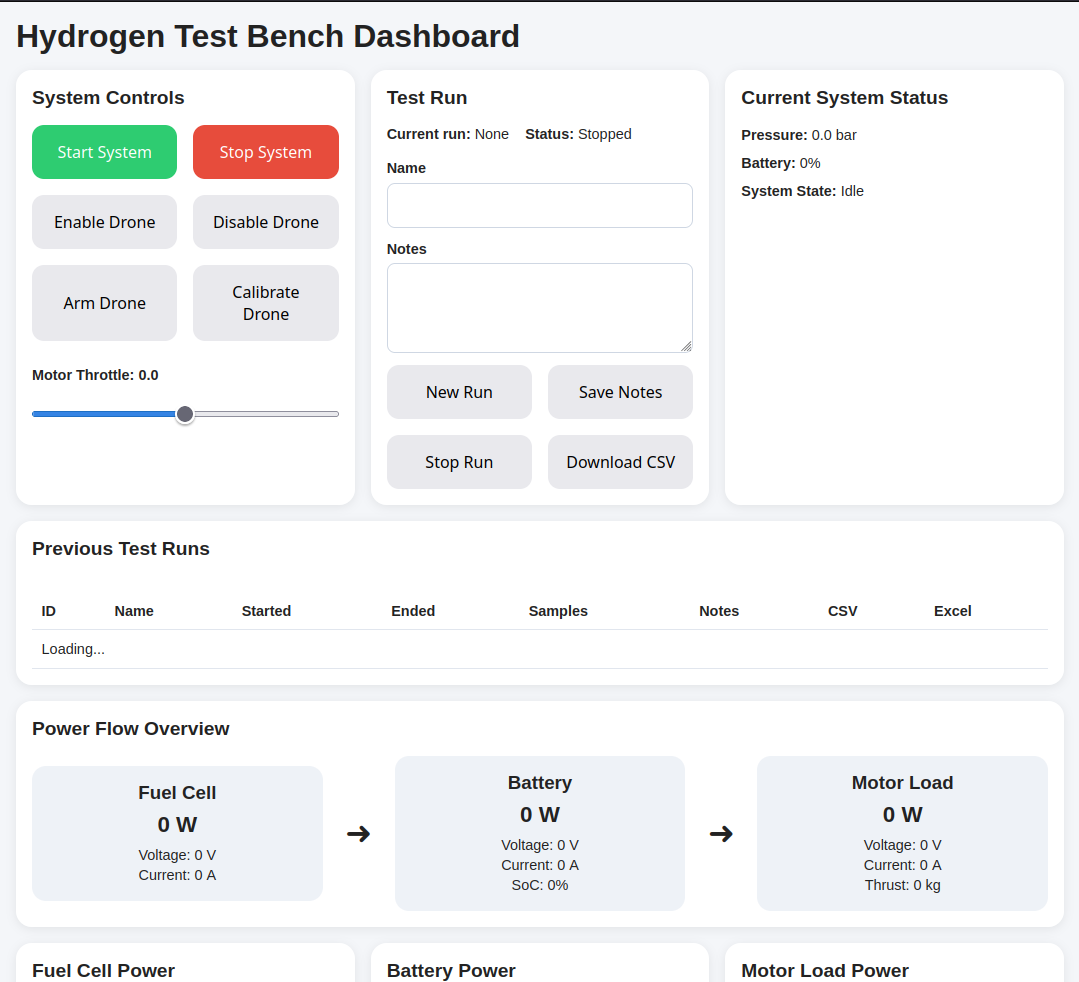
\includegraphics[width=\textwidth]{media/h2_dashboard.png}
    \caption{Webinterface of the Hydrogen Test Setup}
    \label{fig:h2 dashboard}
\end{figure}

\clearpage
